\section{Methodology}
\label{S:meth}
Pedestrian wait time before they start crossing can be modelled as the time it takes before an event occurs. Thus, survival analysis is a popular and powerful tool used for this purpose. In the following, first traditional survival models, and in particular, Cox Proportional Hazards (CPH) models are explained. We used CPH as the base model for comparison in this study. Then, the data-driven deep neural network version of CPH is proposed as the framework used in this study, which enables incorporating more covariates while increasing goodness of fit. Finally, interpretability mechanism used to explain model results and obtain practical implications is outlined.
\subsection{Survival analysis}
Survival analysis techniques are used in cases the time to occurrence of an event is of interest. Although originally developed for applications in medical science where the event is treatment of a disease or the death of the patients, survival methods have found their way in other fields, including transportation. By defining \textit{survival function} $S(t)$ as the probability that the event occurs after time $t$, and \textit{hazard function} $h(t)$ as the probability of the event occurring at time $t$, the following relationship can be established between the two:
\begin{linenomath}
\begin{equation}
\label{eq:1}
    S(t)=\exp({-\displaystyle \int_{0}^{t} h(z) dz)}
\end{equation}
\end{linenomath}
Different methods have been proposed for estimating hazard function, parametric, semi-parametric and non-parametric. Among them, Cox Proportional Hazards (CPH) model is probably the most widely used one, which enables considering the effects of covariates on the hazard function~\citep{cox1972regression}. Equation \ref{eq:2} shows the hazard function formula in CPH.
\begin{linenomath}
\begin{equation}
\label{eq:2}
    h(t|Z)=h_0(t) \times \exp({\displaystyle \sum_{i} \beta_i Z_i})
\end{equation}
\end{linenomath}
In the above equation, $h_0(t)$ is the baseline hazard, which is the hazard function regardless of the values of the covariates and is a function of time, and $\beta_i$ and $Z_i$ are the coefficient and value of covariate $i$, respectively~\citep{therneau2013modeling}. In the terminology of survival analysis, ${e^{\textstyle \sum_{i} \beta_i Z_i}}$ is called partial hazard function or risk function, which is representative of the effects of values of covariates on the hazard function and is independent of time. As it can be seen in equation ~\ref{eq:2}, the log-partial hazard function in CPH is in a linear combination of covariates. To find the coefficients in CPH, the partial likelihood shown in equation~\ref{eq:3} is maximized.
\begin{linenomath}
\begin{equation}
\label{eq:3}
\mathcal{L}(\beta) = \prod_{k\in instances}{\exp({\displaystyle \sum_{i} \beta_i Z_{ik}})} / {\displaystyle \sum_{j: T_j > T_k} \exp({\displaystyle  \sum_{i} \beta_i Z_{ij}})}
\end{equation}
\end{linenomath}
Where, index $j$ in the denominator selects the instances that are still at risk when event of instance $k$ occurs. In this study, we use CPH with linear log-partial hazard function as the base model, in which an event is defined as initiation of a cross by a participant. The simplistic assumption of linearity of log-partial hazard function is what drives us to improve and update the model to account for today's complex data and advanced modelling tools available.  
\subsection{Data-driven survival analysis}
Rapid and ubiquitous emergence of data-driven approaches in recent years provides an opportunity to further improve the models for survival analysis. Due to the availability of complex and high-dimensional data today, traditional methods may not be capable of capturing nonlinearities within data. Thus, we build upon the classic CPH (Equation \ref{eq:2}) and replace the linear log-partial hazard function ($\ \sum_{i}\beta_i Z_i$) with a deep neural network, $g(w)$ \citep{kalatian2019deepwait}. The proposed framework used in this study is outlined in \cref{fig:framework}, and the model components are explained in the next two subsections.

\begin{figure}
    \centering
    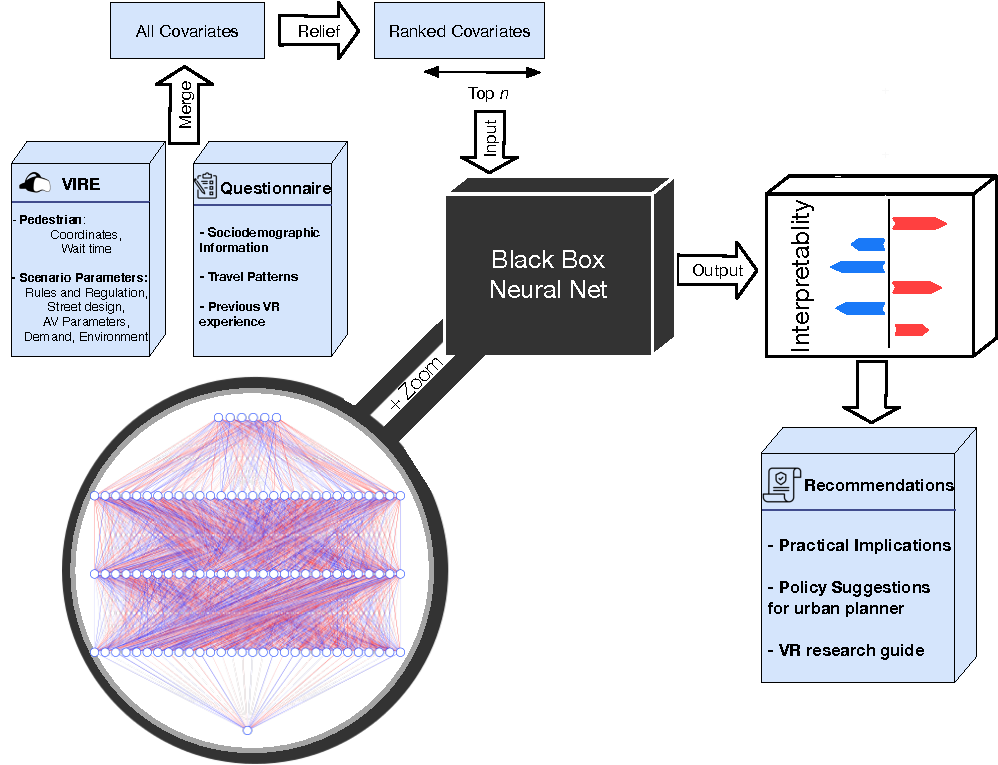
\includegraphics[scale=0.85]{chapter_4/figures/framework.pdf}
    \caption{Framework of the study}
    \label{fig:framework}
\end{figure}

\subsubsection{Feature importance ranking}
High-dimensionality of modern data sources has led researchers and machine learning engineers to incorporate feature selection methods to prevent overfitting and performance degradation~\citep{alelyani2018feature}.  Although deep neural networks are known for their capability of detecting correlation among features, a Variance Inflation Factor (VIF) analysis and feature selection algorithm is implemented in the preprocessing step to 1. develop a base case cox proportional hazards model, and 2. compare the effectiveness of deep survival models with and without data preprocessing.   

Initially proposed by \cite{kononenko1997overcoming} for classification, Relief family of algorithms consider the ability of variables to distinguish among instances that are close to each other,and rank their quality based upon this ability. RRELIEFF~\citep{robnik1997adaptation}, which is an adaptation of Relief for using in regression, is used in this study to prioritize covariates, and reduce the dimensionality of the dataset collected. Based on Relief in its simplest form, the importance of a covariate in a classification task increases, if its value is different for instances from different classes, and decreases if its value is different for instances of the same class. RreliefF, which is the regression version of the family, replaces the classes with a probability defined based on the relative distance between the target values of the instances. In mathematical terms, importance weight of covariate $f$, $W_f$, is calculated based on the following equation~\citep{robnik2003theoretical}:
\begin{linenomath}
\begin{equation}
\label{relief}
    W_f = ({P_{v|f}\times P_f})/{P_v}  - ({(1-P_{v|f})\times P_f})/({1-P_v})
\end{equation}
\end{linenomath}
Where:
\begin{itemize}
    \item $P_f$ = P(different value of $f$ in nearest instances)
    \item $P_v$ = P(different target value in nearest instances)
\end{itemize}
\subsubsection{Hazard function}
The formulation of modified hazard function in our proposed model is shown in equation~\ref{eq:5}:
\begin{linenomath}
\begin{equation}
\label{eq:5}
    h(t|Z)=h_0(t) \times \exp({g_w(Z)})
\end{equation}
\end{linenomath}
where $g_w$ is the dense neural network with weights $w$. Top $n$ covariates ($Z_n$), based on the feature importance ranking, will be imported into the network's input layer.  After a number of fully connected hidden layers, each followed by dropout layers and batch normalization to prevent overfitting to the training data, the output of the network $g(Z_n)$ will be calculated as the value of the last one-node layer, and will be used as our estimation of log-partial hazard. 

In the deep network described, network architecture parameters i.e. number of covariates to be selected, number of hidden layers, number of nodes in each layer and dropout rate as well as optimization parameters, including learning rate decay and momentum, are used as the hyperparameters to be found. The loss function to be minimized in network training is derived from the partial likelihood function of CPH. As shown in equation~\ref{eq:6}, network's loss function would be the average negative logarithm of CPH's partial likelihood:
\begin{linenomath}
\begin{equation}
\label{eq:6}
L_w=-({1}/{N})\times \displaystyle \sum_{k\in instances} \left(g_w(Z_{nk}) - \log\displaystyle  \sum_{j: T_j > T_k} \exp({g_w(Z_{nj})}) \right)     
\end{equation}
\end{linenomath}
where $N$ is the total number of events or instances, and $Z_{nk}$ is the is the value of top $n$ covariates for instance $k$.

\subsection{Model interpretability}
Transition from regression models to neural-based models comes with the cost of losing useful information pertaining to the effects of covariates on the model output. Within traditional CPH models, the effect of each covariate on the log-partial hazard function can be estimated by looking into covariate coefficients. A greater coefficient for a covariate means an increase in log-partial hazard function, and subsequently in hazard function. In other words, a positive coefficient for a covariate means that greater value of that covariate results in higher probability of the event to occur at any time, thus a shorter wait time. By using z-scores and p-values, the significance of variables can be measured in traditional based CPH models. The case is different for neural networks, however, as it is impossible to track the nonlinearities involving multiple variables at the same time and in different layers. 

To address this issue, SHAP (SHapley Additive exPlanations) is used in this study. Introduced in \citep{lundberg2017unified}, SHAP is a game theoretic model explanation method based on Shapley Values. In game theory, Shapley value is a method to \textit{fairly} distribute the payoff of a job done by a coalition of players with different skills, to the players. By replacing the payoff with model prediction and players with features, SHAP calculates the average marginal contribution of each feature to model prediction for each instance. In mathematical terms, Shapley value of each feature $i$ is calculated by equation~\ref{eq:7} as follows~\citep{lipovetsky2001analysis}:
\begin{linenomath}
\begin{equation}
\label{eq:7}
\Phi_i = \sum_{S \in F \setminus \{i\}} \frac{|S|! (|F| - |S| -1)!}{|F|!} \left(
g_{S\cup\{i\}}(Z_{S\cup\{i\}}) - g_S(Z_S) \right)
\end{equation}
\end{linenomath}
In which $S$ is a subset of all features $F$, $g_{S\cup\{i\}}$ is the model trained using a subset with feature $\{i\}$ present, and $g_S$ is the model trained with the feature $i$ missing. One of the advantages of using Shapley values over other interpretation methods is that it considers the fact that the contribution of a feature depends on the values of other features, thus the contributions are computed for all possible subsets. In their paper, \citet{lundberg2017unified} show that SHAP solution satisfies required conditions to fairly distribute the payoff to players. By using Shapley values, importance of the features can be estimated as the average absolute Shapley values of features over the whole instances. 